\documentclass[titlepage]{article}
\usepackage{xcolor} % for different colour comments
\usepackage[left=15mm,right=15mm,top=1in,bottom=1in]{geometry}
\usepackage{framed}
\usepackage{graphicx}
\usepackage{color}
\usepackage{float}
\usepackage{lipsum}
\graphicspath{ {images/} }
%% Comments
\newif\ifcomments\commentsfalse %i replaced comments true by comment false so the comments will be hidden

\ifcomments
\newcommand{\authornote}[3]{\textcolor{#1}{[#3 ---#2]}}
\newcommand{\todo}[1]{\textcolor{red}{[TODO: #1]}}
\else
\newcommand{\authornote}[3]{}
\newcommand{\todo}[1]{}
\fi

\newcommand{\wss}[1]{\authornote{magenta}{SS}{#1}}
\newcommand{\hm}[1]{\authornote{blue}{HM}{#1}} %Hediyeh
\newcommand{\tz}[1]{\authornote{blue}{TZ}{#1}} %Tahereh
\newcommand{\pl}[1]{\authornote{blue}{PL}{#1}} %Peng


\begin{document}
\title{WebHandyTool \\
 Problem Statement : newAGEtech, Group H }
\author{Genevieve Okon (Okong), Abraham Omorogbe(Omorogoa),\\
 Eric Le Forte(Leforte)}
\date{\today}
\maketitle

%\texttt{color} package%
\tableofcontents
\listoffigures
\listoftables

%\textbf{Revision History} \\ \normalsize
%First Draft October 10th 2015\\
%Revision0 Draft October 10th 2015\\
%\clearpage

%\textbf{Revision History} \\ \normalsize
\pagebreak


%%
\section{Revision History}
\textcolor{red}{Red, means changes made in section}
\begin{table}[h!]
	\begin{tabular}{| p{5cm} | p{5cm} | p{5cm} |p{5cm} |}    \hline
Revision  &Revision Date &Description of Change &Author\\ \hline
1& 10-10-15&First Draft&Abraham Omorogbe\\ \hline
2& 10-10-15& Revision 0 Draft&Genevieve Okon\\ \hline
4& 26-11-15& Revised section product use case list &Eric Le Fort\\ \hline
5& 26-11-15& Revised section  individual product use case Number 6&Genevieve Okon\\ \hline
6& 26-11-15& Revised section Functional and data requirements, Requirement 6&Genevieve Okon\\ \hline
7& 26-11-15& Revised section The scope of the  product, The use case diagram &Genevieve Okon\\ \hline

       \end{tabular}
       
       \caption{Revision History}
       \label{table:Revision History}
\end{table}
%%%

\addcontentsline{toc}{section}{Project Drivers}

\section *{Template Used}
This document makes usage of the Volere Template for all its organization



\section{The Purpose of the Project}

\subsection*{The User Business or Background of the Project}
This project will be an attempt to ease the difficult and tedious process of verifying a website’s current status and state of availability. As well as being able to assist researchers in scouring the web efficiently for potentially relevant sources of data. Some specific tasks expected to be completed using this software include ensuring all of a website’s pages are functioning correctly and resources that should be available are, data mining for certain research topics and for security professionals ensuring that only the webpages that should be visible are.

\subsection*{Goals of the Project}
This product aims to be used as an effective tool dealing with various forms of website analysis. It will be an efficient and customizable resource that allows you to perform various web crawler based activities on websites in order to increase productivity and for businesses to save money.


\section{Clients, Customers, Stakeholders}

\subsection*{The Client}
The clients of this product will primarily be analysts and website developers.

\subsection*{The Customer}
The customers of this product will be the companies who employ the aforementioned clients as well as the clients themselves if it is purchased for personal use.

\subsection*{Other Stakeholders}
The other stakeholders include the developers of the software, investors as well as a previously established application store (i.e. Google Play or Apple’s App Store) for distribution.

\section{Users of the Product}

\subsection*{The Hands-On Users of the Product}
Software Developers/Testers\\
- Develops, tests and maintains websites.\\
- Strong knowledge of technology, especially technology involved in this product’s field.\\
- Reasonably educated (most likely a college degree or better).
- Anticipated age group: 20+\\

Researchers\\
- Researches various topics relevant to their business, especially matters pertaining to the stock trade.\\
- No required technological knowledge other than the basics of how to use a computer.\\
- Expected education is a high school diploma or better\\
- Anticipated age group: 20+\\

Other Members of the General Population
- May have any sort of experience, education and skill sets.\\
- Anticipated age group: 10+.\\


\subsection*{Priorities Assigned to Users}
Key Users:\\
- Software Developers/Testers\\
- Researchers\\

Secondary Users:\\
N/A\\

Unimportant Users:\\
- Other Members of the General Population\\

\subsection*{User Participation}
Software Developers:\\
N/A\\

Researchers:\\
- It would be mutually beneficial to obtain a set of desired functionalities that would assist this user in utilizing this product.\\

Other Members of the General Population:\\
N/A

\subsection*{Maintenance Users and Service Technicians}
N/A

\addcontentsline{toc}{section}{Project Constraints}

\section{Mandated Constraints}

\subsection*{Solution Constraints}
	This project will be implemented using the Python programming language. This is due to the language’s simplicity and available libraries related to the project.

\subsection*{Implementation Environment of the Current System}
This product will be installed onto a computer system using any platform that accepts the use of Python and will utilize the architecture of the world wide web.

\subsection*{Partner or Collabrative Applications}
This product will be capable of operating on websites that are locally stored.

\subsection*{Off-The-Shelf Software}
Some example of similar existing solutions include search engines (i.e. Google or Bing), and various other generic web crawlers that have already been implemented.

\subsection*{Anticipated Workplace Environment}
This project is expected to be utilized primarily in office environments. These will include a computer that is likely hooked up to an active internet connection.

\subsection*{Schedule Constraints}
This project must be completed by the eleventh of November.

\subsection*{Budget Constraints}
The budget for this project is exactly \$0.


\section{Naming Conventions \& Defintions}

\subsection*{Definition of All Terms, Including Acronyms, Used in the Project}
Web Crawler/Crawler - An internet bot which systematically browses the World Wide Web, typically for the purpose of Web indexing.
\\
Uniform Resource Locator (URL) - A reference (address) to a resource on the internet. Has two main components: a Protocol Identifier (e.g. http) and a Resource Name (e.g. Google.ca)
\\
HyperText Markup Language (HTML) - The standard markup language used to create webpages.
\\
List of standard HTTP status codes and their definitions:
\\
1XX are informational status codes.
\\
Continue (100) - The client should continue with its request.
\\
Switching Protocols (101) - The server has acknowledged and approved a request to switch protocols.
\\
2xx refers to successful requests.
\\
OK (200) - The request has succeeded.
\\
Created (201) - The request succeeded and resulted in a new resource being created.
\\
Accepted (202) - The request has been approved but is still processing.
\\
Non-Authoritative Information (203) - The returned metadata in the entity-header is not the definitive set defined in the origin server, instead it is gathered from a local or third-party copy.
\\
No Content (204) - Request succeeded but no entity-body was required from the server.
\\
Reset Content (205) - Request succeeded, the document view which caused the request to be sent should be updated.
\\
Partial Content (206) - Partial GET request succeeded.
\\
3xx refers to redirection status codes.
\\
Multiple Choices (300) - The requested resource corresponds to any one of a set of representations.
\\
Moved Permanently (301) - The requested resource has been assigned a new permanent URL.
\\
Found (302) - The requested resource currently resides in a temporary location.
\\
See Other (303) - The response to the request can be found under a different URL and should be retrieved using a GET method on that resource.
\\
Not Modified (304) - The client performed a conditional GET request but the document has not been modified.
\\
Use Proxy (305) - The requested resource must be accessed through the proxy given by the Location field.
\\
(306) - No longer in use, the code is now reserved.∂
\\
Temporary Redirect (307) - The requested resource temporarily resides under a different URL.
\\
4xx refers to Client Error status codes.
\\
Bad Request (400) - The request was not understood due to malformed syntax.
\\
Unauthorized (401) - The request requires user authorization.
\\
Payment Required (402) - Code reserved for future use.
\\
Forbidden (403) - The request was understood however, the server is refusing to fulfill it.
\\
Not Found (404) - The server could not find anything matching the provided URL.
\\
Method Not Allowed (405) - The method specified in the Request-Line is not allowed for the resource identified by the Request-URI.
\\
Not Acceptable (406) - The resource identified by the request is only capable of generating response entities which have content characteristics not acceptable according to the accept headers sent in the request.
\\
Proxy Authentication Required (407) - Similar to 401 except the client must first authenticate itself with the proxy.
\\
Request Timeout (408) - The client did not produce a request within the time that the server was prepared to wait.
\\
Conflict (409) - The request could not be completed due to a conflict with the current state of the resource.
\\
Gone (410) - The requested resource is no longer available at the server and no forwarding address is known.
\\
Length Required (411) - The server refuses to accept the request without a defined content length.
\\
Precondition Failed (412) - The precondition given in one or more of the request header fields evaluated to false when it was tested on the server. 
\\
Request Entity Too Large (413) - The server is refusing to process a request because the request entity is larger than the server is willing or able to process.
\\
Request URL Too Long (414) - The server is refusing to service the request because the request URI is longer than the server is willing to interpret.
\\
Unsupported Media Type (415) - The server is refusing to service the request because the entity of the request is in a format not supported by the requested resource for the requested method.
\\
Requested Range Not Satisfiable (416) - A request included a range request header field and none of the range-specifier values in this field overlap the current extent of the selected resource and the request did not include and if-range request header field.
\\
Expectation Failed (417) - The expectation given in an expect request header field could not be met by this server
\\
5xx refers to Server Error status codes.
\\
Internal Server Error (500) - The server encountered an unexpected condition which prevented it from fulfilling the request.
\\
Not Implemented (501) - The server does not support the functionality required to fulfill the request.
\\
Bad Gateway (502) - The server, while acting as a gateway or proxy, received an invalid response from the upstream server it accessed in attempting to fulfill the request.
\\
Service Unavailable (503) - The server is currently unable to handle the request due to a temporary overloading or maintenance of the server.
\\
Gateway Timeout (504) - The server, while acting as a gateway or proxy, did not receive a timely response from the upstream server specified by the URL it needed to access in attempting to complete the request.
\\
HTTP Version Not Supported (505) - The server does not support, or refuses to support, the HTTP protocol version that was used in the request message.
\\
\subsection*{Data Dictionary for Any Included Models}
This section to be updated as relevant models arise.

\section{Relevant Facts \& Assumptions}

\subsection*{Facts}
The existing solution is 7,000 lines of Python code.

\subsection*{Assumptions}
This product assumes that the operational environment supports the execution of Python code.
This product will assume that the HTML code being parsed for links uses correct syntax (otherwise the error messages may be nonsensical).

\addcontentsline{toc}{section}{Functional Requirements}
\section{The Scope of the Work }

\subsection*{The Current Situation}

It is difficult often difficult for users of the internet to navigates through the web, it can be difficult to locate pertinent information using standard methods of search such as search engines. A web crawler and link validator will allow users quickly traverse the web and quickly and effectively locate information from different web pages and information about these web pages. A web crawler and link validator will increase users efficiency, it will be able to save money and resources due to users spending less time and effort surfing the web for information.\newline

\subsection*{The Context of the Work }
The figure \ref{figure:work context} is a Use case Diagram and the product boundary.
\begin{figure}[h!]
  \caption{Work Context Diagram}
  \centering
    \includegraphics[scale=0.6]{Work_Context_Diagram}
\end{figure}
\label{figure:work context}
\subsection*{Work Partitioning}
The table \ref{table:Business Event List} is a Business Event List.

\begin{table}[H]
    \begin{tabular}{| p{5cm} | p{5cm} | p{5cm} |}    \hline
    Event Name &	Input and Output	 & Summary\\ \hline
    User requests information about a website	& Website start link to crawl and specific info gathering setting (In)	& Have a starting point for crawler can gather resources from. \\ \hline
    User requests information from a website	 & Website start link to crawl and specific status checking setting (In)	& Have a starting point for crawler, it can continue to verify any links associate with initial website.\\ \hline
    Traverse website	& Links from initial retrieved website (In)	& Has the abilities to reach website that are associated with starting link \\ \hline
    
    List of crawled websites status code & 	A list of all the site that were visited (Out)	& Has the ability to show the user the status codes from crawled websites, can verify if links are down. \\ \hline
     
      List of information from website	& All resources from a website (Out)	& Has the ability to show the user all the information from website they have elected. \\ \hline
      
    \end{tabular}
    \caption{Business Event List}
\label{table:Business Event List}
\end{table}
\lipsum[7]


\section{The Scope of the Product}
\subsection*{Product Boundary}
The figure \ref{figure:use case} is a Use case Diagram and the product boundary.
\begin{figure}[H]
  \caption{Use case Diagram and the product boundary}
  \centering
    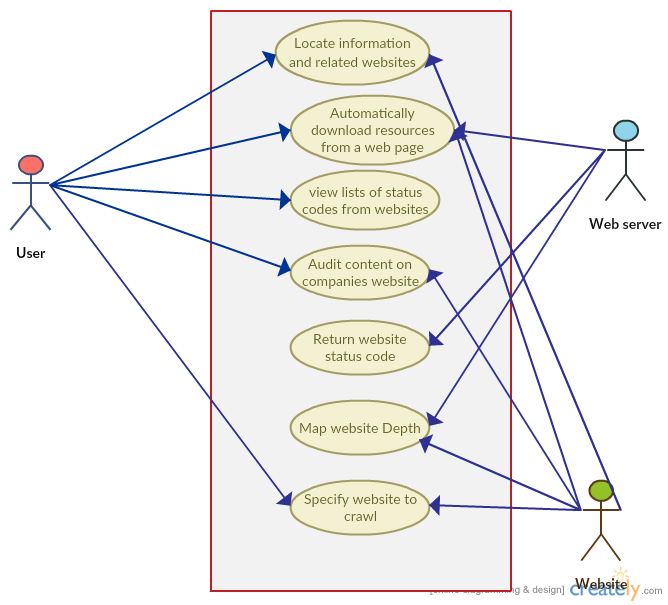
\includegraphics[scale=0.75]{pylinkvalidator_Use_Case_Diagram_copy}
\end{figure}
\lipsum[8]
\label{figure:use case}

\subsection*{Product Use Case List  }
\begin{itemize}
  \item Locate Information and related websites
  \item Automatically download resources from a web page
  \item View list of status codes from website 
  \item Specify website to crawl
  \item Audit Content on companies website 
  \item \textcolor{red}{Map website Depth}
  \item Return website status code
\end{itemize}




\subsection*{Individual Product Use Cases  }
\begin{enumerate}
  \item  Product Use Case Name: Locate Information and related websites \\
  Trigger: User requests a website to be processed \\
Preconditions: User has to specify website that exists\\
Interested Stakeholders: Researchers\\
Actors: User, Website\\
Outcome: If the website is a valid HTML page, the link on the page a verified and information is gathered (text-based), if the website is an invalid, an error is displayed.\\
  \item Product Use Case Name: Automatically download resources from a web page.\\
  Trigger: User types in command to download data
Preconditions: Web server has to have existing resources available, and user needs permission to the website.\\
Interested Stakeholders: Researchers and companies\\
Actors: User, Web Server, Website\\
Outcome: User has all the resources from the website (images, attached files etc.).\\
  \item Product Use Case Name: View list of status codes from website\\
  Trigger: User types in command to show status code\\
Preconditions: User must have Internet connection and must have entered a valid URL.\\
Interested Stakeholders: Developers\\
Actors: User\\
Outcome: User can see a list of all the status codes on websites associated with the initial site.\\
  \item Product Use Case Name: Specify website to crawl\\
Trigger: User types in a website to crawl\\
Preconditions: User must have Internet connection and a valid website to crawl.\\
Interested Stakeholders: Developers\\
Actors User, Website\\
Outcome: The web crawler begins to traverse through website.\\
  \item Product Use Case Name: Audit Content on companies website \\
Trigger: User requests a list of all websites associated with the starting point.\\
Preconditions: User must enter a website with valid $<$a href= "\ldots"$>$ $<$/a$>$ tags\\
Interested Stakeholders: Companies and Developers\\
Actors: User, Website\\
Outcome: The users can see a list of on the links and resources attached to every webpage associated with the specified domain.\\
  \item \textcolor{red}{ Product Use Case Name: Map website Depth\\
Trigger: User requests depth of the website\\
Preconditions: Must have entered a valid URL/HTML.\\
Interested Stakeholders: Researchers, Developers and companies\\
Actors: Web Server, Website\\
Outcome: User is shown the website Depth.\\}
  \item Product Use Case Name: Return website status code\\
Trigger: Web crawler sends request query to web server\\
Preconditions: Web server must respond to queries with status codes. \\
Interested Stakeholders: Developers\\
Actors: Web Server\\
Outcome: The web server responds with correct status code.\\
\end{enumerate}

\section{Functional and Data Requirements}

\subsection*{Functional Requirements}

\begin{framed}

\textbf{Requirement \#}: 1 \hfill \textbf{Requirement Type}: 9 \hfill\textbf{Event/Use case \#}: 7 \hfill\\
\textbf{Description}:  The product shall return the status code of websites\\
\textbf{Rationale}: To allow the users verify the status of all the pages on a website. Checks if it is offline, Unauthorized etc.\\
\textbf{Originator}: Abraham Omorogbe\\
\textbf{Fit Criterion}: The web crawler displays an error with it reaches an website that is not online (Status Code: 200 ) and the status code related the error (Status Code: 400,500 etc.).	\\
\textbf{Customer Satisfaction}: 5 \hfill 	\textbf{Customer Dissatisfaction}: 5 \hfill\\
\textbf{Priority}: High \hfill \textbf{Conflicts}: None \hfill 		\\
\textbf{Supporting Material}: None\\
\textbf{History}: Created October 9, 2015 \hfill	 \textbf{Volere}\hfill

\end{framed}

\begin{framed}
\textbf{Requirement \#}: 2 \hfill \textbf{Requirement Type}: 9 \hfill\textbf{Event/Use case \#}: 2 \hfill\\
\textbf{Description}:  The product shall download resources from a website\\
\textbf{Rationale}: To allow users quickly download all the HTML, images, CSS and other data related to a website\\
\textbf{Originator}: Abraham Omorogbe\\
\textbf{Fit Criterion}:  The download resources can be retrieved and used.\\
\textbf{Customer Satisfaction}: 5 \hfill 	\textbf{Customer Dissatisfaction}: 5 \hfill\\
\textbf{Priority}: High \hfill \textbf{Conflicts}: None \hfill 		\\
\textbf{Supporting Material}: None\\
\textbf{History}: Created October 9, 2015 \hfill	 \textbf{Volere}\hfill

\end{framed}

\begin{framed}
\textbf{Requirement \#}: 3 \hfill \textbf{Requirement Type}: 9 \hfill\textbf{Event/Use case \#}: 1,5 \hfill\\
\textbf{Description}:  The product shall have adjustable search max-depth\\
\textbf{Rationale}: To allow the user specific how many layers of the website, the user want to analyse. Helps with auditing and finding related sites.\\
\textbf{Originator}: Abraham Omorogbe\\
\textbf{Fit Criterion}: The web crawler only show top-level links when max-depth is at 0, and shows more levels of the website when depth $\geq$ 1\\
\textbf{Customer Satisfaction}: 5 \hfill 	\textbf{Customer Dissatisfaction}: 5 \hfill\\
\textbf{Priority}: High \hfill \textbf{Conflicts}: None \hfill \\
\textbf{Supporting Material}: None\\
\textbf{History}: Created October 9, 2015 \hfill	 \textbf{Volere}\hfill

\end{framed}

\begin{framed}
\textbf{Requirement \#}: 4 \hfill \textbf{Requirement Type}: 9 \hfill\textbf{Event/Use case \#}: 4 \hfill\\
\textbf{Description}:  The product shall always users enter a starting URL or local HTML page\\
\textbf{Rationale}: To allow the user crawl any website that is on or offline\\
\textbf{Originator}: Abraham Omorogbe\\
\textbf{Fit Criterion}: The crawler starts from the inputted website.\\
\textbf{Customer Satisfaction}: 5 \hfill 	\textbf{Customer Dissatisfaction}: 5 \hfill\\
\textbf{Priority}: High \hfill \textbf{Conflicts}: None \hfill 		\\
\textbf{Supporting Material}: None\\
\textbf{History}: Created October 9, 2015 \hfill	 \textbf{Volere}\hfill

\end{framed}

\begin{framed}
\textbf{Requirement \#}: 5 \hfill \textbf{Requirement Type}: 9 \hfill\textbf{Event/Use case \#}: 3,5 \hfill\\
\textbf{Description}:  The product shall display all a report of all found results and corresponding websites\\
\textbf{Rationale}: This is one of the main functionality of a web crawl, the application should be able to start at one sites and find related links. List will be used to gather info and check status codes	\\
\textbf{Originator}: Abraham Omorogbe\\
\textbf{Fit Criterion}: The reports are accurate. All link that are reported as status code 404 are offline and all details of resource match source website.\\
\textbf{Customer Satisfaction}: 5 \hfill 	\textbf{Customer Dissatisfaction}: 5 \hfill\\
\textbf{Priority}: High \hfill \textbf{Conflicts}: None \hfill 		\\
\textbf{Supporting Material}: None\\
\textbf{History}: Created October 9, 2015 \hfill	 \textbf{Volere}\hfill

\end{framed}

\begin{framed}
\textcolor{red}{
\textbf{Requirement \#}: 6 \hfill \textbf{Requirement Type}: 9 \hfill\textbf{Event/Use case \#}: 5,6 \hfill\\
\textbf{Description}:  The product shall able to display website’s depth\\
\textbf{Rationale}: Give to users a visual representation of the depth for entered website.\\
\textbf{Originator}: Abraham Omorogbe\\
\textbf{Fit Criterion}: The web depth matches the depth of inputted website.	\\
\textbf{Customer Satisfaction}: 5 \hfill 	\textbf{Customer Dissatisfaction}: 5 \hfill\\
\textbf{Priority}: High \hfill \textbf{Conflicts}: None \hfill 		\\
\textbf{Supporting Material}: None\\
\textbf{History}: Created October 9, 2015 \hfill	 \textbf{Volere}\hfill}

\end{framed}

\begin{framed}
\textbf{Requirement \#}: 7 \hfill \textbf{Requirement Type}: 9 \hfill\textbf{Event/Use case \#}: 1 \hfill\\
\textbf{Description}:  The product shall find specific information from specified websites and related sites\\
\textbf{Rationale}: To allow user enter details they are looking for, and the application can return data based on starting URL.\\
\textbf{Originator}: Abraham Omorogbe\\
\textbf{Fit Criterion}: Returned websites most be related with inputted website and information return must match what the user specified.\\
\textbf{Customer Satisfaction}: 5 \hfill 	\textbf{Customer Dissatisfaction}: 5 \hfill\\
\textbf{Priority}: High \hfill \textbf{Conflicts}: None \hfill 		\\
\textbf{Supporting Material}: None\\
\textbf{History}: Created October 9, 2015 \hfill	 \textbf{Volere}\hfill

\end{framed}

\subsection*{Data Requirements}
\begin{itemize}
  \item Valid HTML pages to be parsed and crawl through.
  \item The websites resources that the crawler can download and check for. \\ \\
\end{itemize}


\addcontentsline{toc}{section}{Non-Functional Requirements}
\section{Look and Feel Requirements}

\subsection*{Appearance requirements:}  The command line interface has to be intuitive for all users of the web crawler.

\subsection*{Style requirements: }It would be recommended for users to use our program with a command line interface.

\section{Usability and Humanity Requirements }

\subsection*{Ease of Use Requirements:} Interface of the program should be intuitive and easy to understand. People with no training of the command line interface can use the product.

\subsection*{Personalization and international requirements: }This program can be used by anybody who has access to a computer and has adequate knowledge of a command line.

\subsection*{Learning requirements:}  This program shall be easy to learn by an individual with adequate knowledge of the command line. If the user is using the webcrawler, he/she shall spend no more than a few seconds waiting for the results of the webcrawler depending on the number of links on a website.

\subsection*{Understandability and Politeness Requirement: }The program shall hide the details of its construction from the user.

\subsection*{Accessibility requirements:} A person using the program needs all fingers needed for typing by the user and eyesight. The product shall conform to the Americans with Disabilities Act.

\section{Performance Requirements }

\subsection*{Speed and Latency Requirements:}
Speed of the program depends on the speed of the operating system. The program shall respond to the user's requests within seconds, dependent on the number of links on the webpage. 

\subsection*{Safety-Critical Requirements: }The program should not infringe the user's privacy. 
This will be verified prior to completion of the program.

\subsection*{Precision or Accuracy Requirements:}
The program should specify the type of error accurately. If a link is not working the program should identify that it's not working with the correct error code.

\subsection*{Reliability and Availability Requirements:}

This program should work whenever the user wants to use it - 24 hours a day, 7 days a week.

\subsection*{Robustness or Fault-Tolerance Requirements:}
The system should tolerate corrupted HTML data, unexpected server configurations and behaviours and any other strange issues. Our system detects these situations and makes decisions or provides error messages for the system administration function.
If there is an error found while a webpage is being crawled it should prompt a message stating the error next to the link and continue checking for other links.

\subsection*{Capacity Requirements:}
Each user who's using the web-crawler is independent of another. Therefore there's no limit as to the number of people who can use this program at once.

\subsection*{Scalability or Extensibility Requirements:}
Scalability, in terms of the increasing number of users over time, is not a concern.

\subsection*{Longevity Requirements:}
This program performs a webcrawl on links. So it is reliable until there's a major change in the website are designed and the markup.

\section{Operational and Environmental Requirements }

\subsection*{Expected Physical Environment:}
This program can be used anywhere using a device with suitable software requirements. 

\subsection*{Requirements for Interfacing with Adjacent Systems:}
WebHandyTool(the web-crawler) does not require external libraries if executed with python 2.x. It requires beautifulsoup4 if executed with python 3.x. It has been tested on python 2.6, python 2.7, and python 3.3.


\subsection*{Production Requirements:}

The product shall be distributed as pip. WebHandyTool(the web-crawler) file can be downloaded from Github. It can be used on any device, which has an operating system that can run a python program. The device also needs to have a suitable interface for user interaction (e.g. command line interface).


\subsection*{Release Requirements: }
A new release of the program shall not intervene with the data of the previous program. A webpage can still be crawled with the older version of the program, given the there exists a newer version.

\section{Maintainability and Support Requirements }

\subsection*{Maintenance Requirements:}
 The maintenance of the app has to be done by developers, and end user has no role in this regard.

\subsection*{Supportability Requirements:}

This web-crawler program is self-supporting as its interface is very intuitive.

\subsection*{Adaptability Requirements:}

The product is expected to run on python under Windows XP and Linux, mac os x. 

\section{Security Requirements }

\subsection*{Access Requirements:}
Only the user has access to their own personal information, like the last webpage crawled. The program will not keep track of this information, and developers have no access to it either.

\subsection*{Integrity Requirements:}
This is not applicable since this program does not rely on stored data any result produced comes from the webpage which is crawled. 

\subsection*{Privacy Requirements:}
The product shall notify customers of changes to its information policy.

\subsection*{Audit Requirements:}
Not applicable.

\subsection*{Immunity Requirements:}
Not applicable.

\section{Cultural Requirements}

\subsection*{Cultural Requirements:}

The webcrawler can be used by anyone regardless of his or her cultural background.

\section{Legal Requirements }

\subsection*{Compliance Requirements:}

Not applicable.

\subsubsection*{Standards Requirements:}

The webcrawler complies with all software development standards.\\
\\

\addcontentsline{toc}{section}{Project Issues}
\section{Open Issues }

\begin{itemize}
  \item Parts of user interface not known.
  \item Testing of user interface not known.
  \item Updating user interface.
\end{itemize}


\section{Off-the-Shelf Solutions }
\textbf{Ready-Made Products}:\\ Not applicable.

\subsection*{Reusable Components:}
Not applicable.

\subsection*{Products That Can Be Copied:}
There are other WebCrawlers that are available, which we can use as a foundation for our program. Its specification can cut our analysis effort by a lot.

\section{New Problems }
\textbf{Effects on the Current Environment:}
Not applicable.

\subsection*{Effects on the Installed Systems:}
Not applicable.

\subsection*{Potential User Problems:}
Not applicable.

\subsection*{Limitations in the Anticipated Implementation Environment That May Inhibit the New Product}

Not applicable.

\subsection*{Follow-Up Problems:}
Making changes to the web-crawler as more changes occur 

\section{Tasks} 

\begin{itemize}
  \item Work on prototype and get feedback from supervisor.
  \item Discuss missing requirements and add them.
     \item Revise requirements document.
  \item Create a test plan.
  \item Demonstrate a proof of concept.
  \item Draw up design documents.
  \item Revision 0 project demonstration.
\item Final revision project demonstration.
\end{itemize}

\section{Migration to the New Product }
Not applicable.

\section{Risks }

\subsection*{Loss of Personnel:}The loss of one member would be detrimental due to the size on our small group. Each group member has been assigned tasks of equal value. We are having weekly meetings to share detailed progress reports as a precautionary measure. 

\subsection*{Learning of the software tools:} Some of the software tools are new to the team members, so in order to successfully complete implementation of the program and meet project deadlines it is imperative that the members of the group learn to use these tools in a timely manner.

\section{Costs }
This program is not for profit. There are no direct monetary costs associated with this project.

\section{User Documentation and Training }
User’s will provided with information on program use via a “Help” option which, when selected, will
open a dialog box detailing general functionality of the program along with an FAQ section.

\section{Waiting Room}
New features of this product would include Linux functionality and multiple language support.

\section{Ideas for Solutions}
Not applicable



\noindent \wss{This is an example comment.  You can turn comments off by replacing
  commentstrue by commentsfalse.}\\
\hm{Sample comment}\\
\tz{Sample comment}\\
\pl{Sample comment}

\end{document}